\problemname{Legobyggartävlingen}
Du och din ärkefiende Gohu har deltagit i en legobyggartävling.
Ni har byggt en massa olika höga och olika fina torn längs $x$-axeln och väntar nu på att domarna ska komma.
Poängsättningen kommer gå till enligt följande: Om ett av dina torn har finhetsgraden $f$ och är $h$ legobitar högt kommer du få $f\cdot h$ poäng för tornet.

\begin{figure}[!h]
  \centering
  
\includegraphics[width=6cm]{sample}
  \caption{Bilden motsvarar andra exemplet.}
\end{figure}

Legobyggartävlingen är ett världskänt jippo och det flyger därför en massa drönare fram och tillbaka för att filma alla fina torn.
För att drönarna inte ska krocka med tornen (och därmed riva ner alla legobitar ovanför och inkluderat med legobiten den krockade med) har filmteamet placerat ut en massa radiomaster av olika höjd längs med $x$-axeln.
En drönare kan röra sig en ruta upp eller ned för varje ruta framåt och kommer alltid röra sig så att den ligger så nära marken som möjligt (för att få bra bilder på tornen) utan att någonsin åka under en mast.

Nu plötsligt tittar filmteamet bort!
Du bestämmer dig för att snabbt ta bort några master från linjen så att drönarna ska börja krascha in tornen.
Vilka master ska du ta bort för att maximera din vinst (skillnaden mellan dina poäng och Guhos)?

Finhetsgraden på ett torn minskar inte när en drönare kraschar in i den, bara höjden.
Det är garanterat att masterna initialt är placerade så att drönarna inte krockar med några torn.


\section*{Indata}
Den första raden innehåller tre heltal $A,B,M$ ($1 \leq A,B,M \leq 2000$) -- antalet torn du byggt, antalet torn Guho har byggt och antalet master.

Därefter följer $A$ rader där varje rad innehåller heltal $x,f,h$ ($1 \leq x \leq 10^6, 1 \le f \le 100, 1\leq h \leq 10000$) -- position, finhetsgrad och höjd för ett av dina torn.

Därefter följer $B$ rader där varje rad innehåller heltal $x,f,h$ ($1 \leq x \leq 10^6, 1 \le f \le 100, 1\leq h \leq 10000$) -- position, finhetsgrad och höjd för ett av Guhos torn.

Därefter följer $M$ rader där varje rad innehåller heltal $x,h$ ($1 \leq x \leq 10^6, 1\leq h \leq 10000$) -- position och höjd för en av masterna.

Inga torn kommer ha samma $x$-värde som varandra, och inte heller master.
Däremot kan master ha samma $x$-position som torn.

\section*{Utdata}
Skriv ut ett heltal: det största värdet $(\text{dina poäng}) - (\text{Guhos poäng})$ kan uppnå om du optimalt väljer vilka master att ta bort.

\section*{Poängsättning}
Din lösning kommer att testas på en mängd testfallsgrupper.
För att få poäng för en grupp så måste du klara alla testfall i gruppen.

\noindent
\begin{tabular}{| l | l | p{12cm} |}
  \hline
  Grupp & Poängvärde & Gränser \\ \hline
  $1$   & $23$       & Masterna har lägre x-koordinat än tornen \\ \hline
  $2$   & $10$       & $A,B,M \leq 8$\\ \hline
  $3$   & $22$       & $A,B,M \leq 100$  \\ \hline
  $4$   & $45$       & Inga ytterligare begränsningar  \\ \hline
\end{tabular}

\section*{Förklaring av exempelfall}

\begin{figure}[!h]
  \centering
  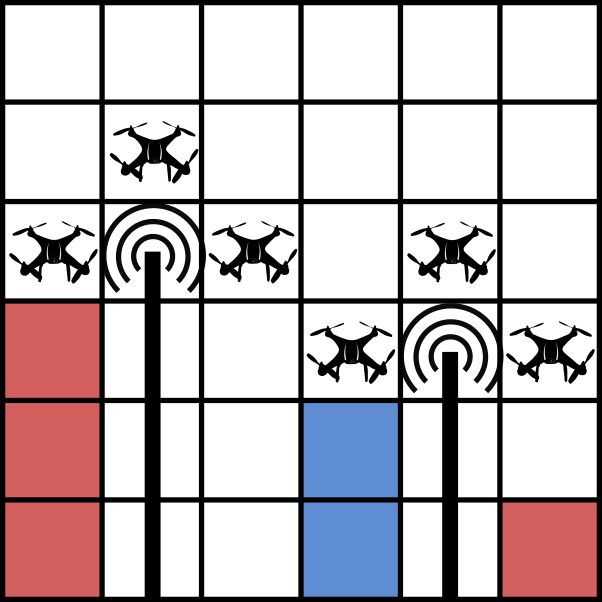
\includegraphics[width=4cm]{sample1.png}
  \caption{Exempelfall 1}
\end{figure}
\begin{figure}[!h]
  \centering
  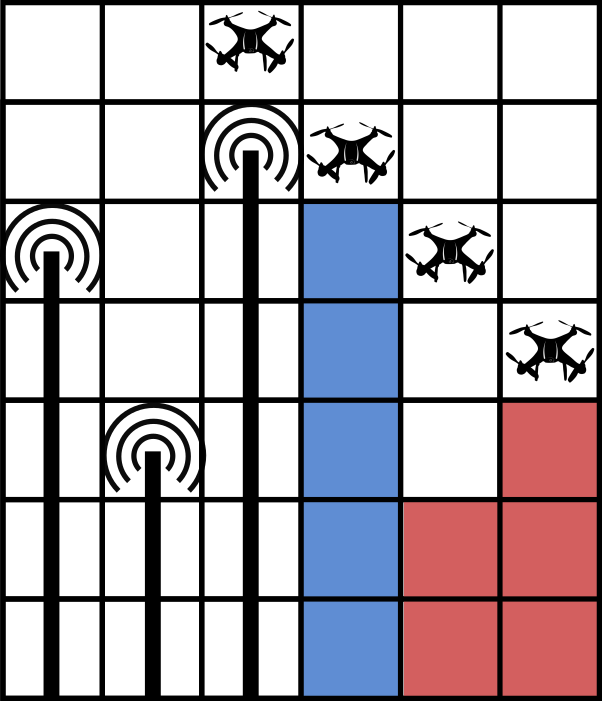
\includegraphics[width=4cm]{sample3.png}
  \caption{Exempelfall 3}
\end{figure}
I alla bilder visas dina torn i blått och Guhos torn i rött.

I det första exempelfallet är det optimalt att bara plocka bort det första tornet. Efter det har du $2$ poäng och Guho har $0+1$ poäng, med en skillnad på $1$ poäng.

I andra exempelfallet är det bästa du kan göra att plocka bort det andra och det tredje tornet. Efter det har du $500+30+120=650$ poäng och Guho har $400+30=430$ poäng, med en skillnad på $220$ poäng.

I det tredje exempelfallet är det optimalt att plocka bort det andra och det tredje tornet. Efter det har du $20$ poäng och Guho har $9$ poäng, med en skillnad på $11$ poäng.
